\documentclass[]{article}
\usepackage{lmodern}
\usepackage{amssymb,amsmath}
\usepackage{ifxetex,ifluatex}
\usepackage{fixltx2e} % provides \textsubscript
\ifnum 0\ifxetex 1\fi\ifluatex 1\fi=0 % if pdftex
  \usepackage[T1]{fontenc}
  \usepackage[utf8]{inputenc}
\else % if luatex or xelatex
  \ifxetex
    \usepackage{mathspec}
  \else
    \usepackage{fontspec}
  \fi
  \defaultfontfeatures{Ligatures=TeX,Scale=MatchLowercase}
\fi
% use upquote if available, for straight quotes in verbatim environments
\IfFileExists{upquote.sty}{\usepackage{upquote}}{}
% use microtype if available
\IfFileExists{microtype.sty}{%
\usepackage{microtype}
\UseMicrotypeSet[protrusion]{basicmath} % disable protrusion for tt fonts
}{}
\usepackage[margin=1in]{geometry}
\usepackage{hyperref}
\hypersetup{unicode=true,
            pdfborder={0 0 0},
            breaklinks=true}
\urlstyle{same}  % don't use monospace font for urls
\usepackage{graphicx,grffile}
\makeatletter
\def\maxwidth{\ifdim\Gin@nat@width>\linewidth\linewidth\else\Gin@nat@width\fi}
\def\maxheight{\ifdim\Gin@nat@height>\textheight\textheight\else\Gin@nat@height\fi}
\makeatother
% Scale images if necessary, so that they will not overflow the page
% margins by default, and it is still possible to overwrite the defaults
% using explicit options in \includegraphics[width, height, ...]{}
\setkeys{Gin}{width=\maxwidth,height=\maxheight,keepaspectratio}
\IfFileExists{parskip.sty}{%
\usepackage{parskip}
}{% else
\setlength{\parindent}{0pt}
\setlength{\parskip}{6pt plus 2pt minus 1pt}
}
\setlength{\emergencystretch}{3em}  % prevent overfull lines
\providecommand{\tightlist}{%
  \setlength{\itemsep}{0pt}\setlength{\parskip}{0pt}}
\setcounter{secnumdepth}{0}
% Redefines (sub)paragraphs to behave more like sections
\ifx\paragraph\undefined\else
\let\oldparagraph\paragraph
\renewcommand{\paragraph}[1]{\oldparagraph{#1}\mbox{}}
\fi
\ifx\subparagraph\undefined\else
\let\oldsubparagraph\subparagraph
\renewcommand{\subparagraph}[1]{\oldsubparagraph{#1}\mbox{}}
\fi

%%% Use protect on footnotes to avoid problems with footnotes in titles
\let\rmarkdownfootnote\footnote%
\def\footnote{\protect\rmarkdownfootnote}

%%% Change title format to be more compact
\usepackage{titling}

% Create subtitle command for use in maketitle
\providecommand{\subtitle}[1]{
  \posttitle{
    \begin{center}\large#1\end{center}
    }
}

\setlength{\droptitle}{-2em}

  \title{}
    \pretitle{\vspace{\droptitle}}
  \posttitle{}
    \author{}
    \preauthor{}\postauthor{}
    \date{}
    \predate{}\postdate{}
  
\usepackage{graphicx,latexsym}
\usepackage{amssymb,amsthm,amsmath}
\usepackage{longtable,booktabs,setspace}

\begin{document}

\section*{Introducción}\label{introduccion}
\addcontentsline{toc}{section}{Introducción}

Las enzimas catalizan reacciones químicas transformando sustratos en
productos. Durante el siglo XX, las enzimas fueron percibidas como
catalizadores altamente específicos, sin embargo, esta percepción cambió
con el descubrimiento de que pueden. Esta capacidad de catalizar varias
funciones químicas se conoce como la promoción de la enzima. Escherichia
coli contiene al menos 404 enzimas promiscuas. La relevancia de la
promiscuidad radica tanto en su papel como mecanismo de evolución de la
funcion enzimatica, asi como en la necesidad de su deteccion para la
correccion de modelos de flujo metabolico y la determinacion de efectos
secundarios en drogas farmacologicas. A pesar de su frecuencia e
importancia aun se esta en el proceso de entender las causas y las
caracteristicas observables de la promiscuidad enzimatica.

Para estudiar la promiscuidad es necesario contar con una definicion,
algunos autores emplean el termino promiscuidad para describir
actividades enzimaticas distintas a la funcion principal
{[}@khersonsky\_enzyme\_2010{]} otros lo ven como una actividad
secundaria fortuita {[}@copley\_enzymes\_2003{]} que pudo aparecer de
forma accidental o inducida artificialmente {[}@hult\_enzyme\_2007{]}.
Otros mas, cuando una enzima puede operar sobre un amplio rango de
sustratos, prefieren llamarla multiespecifica
{[}@khersonsky\_enzyme\_2010{]}. A la accion de realizar distintas
funciones cataliticas, ya sea al catalizar varias reacciones quimicas o
bien una misma reaccion en sustratos diferentes se le conoce como
promiscuidad enzimatica {[}@obrien\_catalytic\_1999{]}. Existen varios
tipos de promiscuidad enzimatica.

Por sustrato cuando la reaccion es la misma pero se lleva a cabo en
distintos sustratos ejemplo la familia PriA
{[}@baronagomez\_occurrence\_2003{]} y la familia de betalactamasas
{[}@risso\_phenotypic\_2014{]}

Catalitica cuando la enzima utiliza diferentes mecanismos de reaccion
y/o residuos cataliticos, e.g.~la quimotripsina puede catalizar
reacciones de amidasa y fosfotriesterasa en un mismo sitio activo.
{[}@obrien\_catalytic\_1999{]} Por condiciones del entorno, cuando la
enzima cambia su conformacion dependiendo de las condiciones quimicas y
fisicas presentes como pH, temperatura, solventes organicos y salinidad
e.g.~algunas lipasas pueden actuar como sintetizadoras de esteres en
lugar de hidrolasas en presencia de solventes organicos
{[}@hult\_enzyme\_2007, @kumari\_preparation\_2007{]}.

Este trabajo se enfocara a la promiscuidad por sustrato, entendiendo asi
que la enzima es capaz de catalizar la misma reaccion quimica en al
menos dos sustratos. La promiscuidad por sustrato es importante en
terminos evolutivos, por ejemplo la enzyme commission number (EC) separa
las enzimas en clases, a cada enzima se asignan 4 digitos, los tres
primeros corresponden a la reaccion y el ultimo al sustrato; el mayor
numero de sustratos (4306 clases) que de reacciones quimicas (234 en el
tercer nivel) sugiere que la mayor variacion evolutiva se da a nivel de
sustrato y no de reaccion {[}@li\_computational\_2004{]}. Otra evidencia
de la importancia de la multiespecificidad por sustrato esta en el
descubrimiento de las superfamilias, enzimas mecanistica y
estructuralmente relacionadas que divergen en su afinidad por sustrato
{[}@glasner\_evolution\_2006, @baier\_evolution\_2016{]}

Si bien existen familias de enzimas con alta especificidad por sustrato,
otras familias como el citocromo P450 {[}@bloom\_neutral\_2007,
@nath\_quantitative\_2008{]} y las beta lactamasas
{[}@zou\_evolution\_2015{]} son promiscuas. Es posible que la vision
previa de alta especificidad se deba a que las primeras rutas
metabolicas estudiadas pertenecen al metabolismo central, donde la
especificidad puede haber sido favorecida por presiones de seleccion
{[}@firn\_darwinian\_2009{]}. Esta vision ha cambiado debido al
conocimiento de mas enzimas con multifuncionalidad
{[}@jia\_multifunctional\_2013{]}, sin afectar la eficiencia catalitica
por la funcion primaria {[}@aharoni\_evolvability\_2005{]}. En 1976 el
interes por la promiscuidad comenzo por su influencia en la evolucion de
la funcion enzimatica{[}@jensen\_enzyme\_1976, @pandya\_enzyme\_2014{]},
las aproximaciones variaron desde la aparicion de la sintesis funcional
{[}@dean\_mechanistic\_2007{]}, cuando la disponibilidad de genomas
permitio la combinacion de analisis filogeneticos con tecnicas de
biologia molecular, bioquimica y biofisica (Fig 1). En 2003 la biofisica
de las proteinas entra en escena al postularse que la diversidad
conformacional durante la dinamica molecular debe incidir en la
aceptacion de distintos sustratos. Recientemente se ha investigado su
papel en efectos secundarios en drogas farmacologicas
{[}@nobeli\_protein\_2009,@hopkins\_drug\_2009,@nath\_quantifying\_2010,@von\_eichborn\_promiscuous:\_2011,
@zhang\_multidimensional\_2012, @zou\_evolution\_2015{]}. Entre 2005 y
2010 se avanza del estudio de una sola familia enzimatica hacia el
interes por propiedades globales, por ejemplo dado un genoma se
investiga la distribucion de familias promiscuas en subsistemas
metabolicos. En estos años, surge el desarrollo de indices que reflejen
las caracteristicas bioquimicas de enzimas promiscuas. En 2010,
comienzan los intentos por desarrollar un metodo computacional de
prediccion de promiscuidad. Desde 2012 a la fecha, a la par que las
aproximaciones bioinformaticas se multiplican, se desarrollan
investigaciones de aspectos biofisicos, bioquimicos y evolutivos de
enzimas promiscuas reafirmando que todos estos aspectos estan
relacionados al fenomeno. En las siguientes secciones se describiran
trabajos importantes sobre la relacion que guarda la promiscuidad con
expansiones genomicas y flexibilidad molecular. Ademas se hablara sobre
analisis bioquimicos y metabolicos para la descripcion del fenomeno.

\subsubsection{Funcion biologica de la promiscuidad
enzimatica}\label{funcion-biologica-de-la-promiscuidad-enzimatica}

¿Por que existe la promiscuidad enzimatica? Se tiene evidencia de dos
papeles biologicos: el primero proporcionar robustez a la red metabolica
de un organismo mediante redundancia de reacciones de otras enzimas; el
segundo permitir plasticidad evolutiva, es decir materia prima para la
adaptacion a variaciones ambientales
{[}@aharoni\_evolvability\_2005,@sanchez-ruiz\_promiscuity\_2012,
@martinez-nunez\_lifestyle\_2015{]} mediante la adquisicion de nuevas
funciones quimicas. Respecto a la robustez, se probo que sobreexpresar
enzimas promiscuas puede rescatar perdidas genicas
{[}@patrick\_multicopy\_2007{]}. De 104 knockout sencillos de genes
esenciales para E. coli K-12, 20\% de las auxotrofias pudieron ser
suprimidas por la sobreexpresion de plasmidos que contenian enzimas
promiscuas. Otro ejemplo que aporta a la robustez es PriA, enzima de la
ruta de histidina que realiza en la ruta del triptofano la reaccion E.C.
5.3.1.24 {[}@baronagomez\_occurrence\_2003{]}. En cuanto a la
plasticidad se propone que para que la promiscuidad pueda dar origen a
la aparicion de nuevas funciones la actividad promiscua debe proveer una
ventaja fisiologica inmediata para poder ser seleccionada positivamente,
ademas una vez que una funcion promiscua se vuelva relevante se debe
poder mejorar mediante pocas mutaciones derivando en el intercambio
entre la actividad promiscua y la
principal{[}@khersonsky\_enzyme\_2010{]}.

Aun cuando el producto de la promiscuidad genera metabolitos que no se
integran al metabolismo central de la celula, su efecto es positivo ya
que estos metabolitos podrian colaborar a la adaptacion al entorno
participando por ejemplo en una relacion de simbiosis o de competencia
con otros organismos. Este tipo de metabolitos, por lo general, no son
dañinos {[}@notebaart\_network-level\_2014, @linster\_metabolite\_2013,
@khanal\_differential\_2015{]} y pueden servir como bloques de
construccion para vias metabolicas nuevas {[}@ma\_unconventional\_2013,
@adams\_promiscuous\_2014, @soskine\_mutational\_2010{]}. La respuesta
inmediata de adaptacion de un organismo podria ser una consecuencia de
su grado de promiscuidad.

\subsubsection{Relacion del pangenoma con la promiscuidad
enzimatica}\label{relacion-del-pangenoma-con-la-promiscuidad-enzimatica}

El pangenoma es el contenido génico total de un linaje taxonómico. Las
familias génicas de un pangenoma pueden clasificarse según su frecuencia
de presencia/ausencia en cada genoma del linaje. De acuerdo a esta
clasificación los principales grupos de familias génicas en un pangenoma
son el \emph{core}, el \emph{shell} y el \emph{cloud} también conocido
como \emph{dispensable} o \emph{accesory}\$\_ genome. El \emph{core
genome} es el conjunto de familias con presencia en todos los genomas
del linaje. Por ejemplo, tanto la secuencia de la subunidad 16s de rRNA
así como los diversos genes ribosomales suelen estar en el \emph{core}
de la gran mayoría de linajes bacterianos. El \emph{shell genome} es el
grupo de familias presentes en la mayoría de los genomas pero no en
todos. En el \emph{shell} se ubican por ejemplo familias que estaban en
el \emph{core genome} pero que algunas bacterias del linaje sufrieron
una dinámica de pérdida génica. Mientras que el \emph{cloud genome} o
\emph{dispensable genome} es aquel grupo de familias que sólo ocurre en
unos cuantos genomas del linaje.

En el Dominio Bacteria se estima que entre al rededor de 200 secuencias
están altamente conservadas. Si bien no están en el \(core\), estas
secuencias están compartidas por 90\% de los genomas
{[}@halachev\_calculating\_2011{]}. El \emph{core} depende de los
genomas seleccionados, entre menos amplio sea el rango filogenético
electo mayor será el tamaño del \(core\). Dada su conservacion el
\(core~genome\) puede utilizarse para trazar mejores relaciones
filogeneticas que las obtenidas con el uso exclusivo de marcadores como
la subunidad 16s del RNA ribosomal o el gen rpoB. El pangenoma es el
conjunto complemento del core genome, es decir todas aquellas secuencias
que estan ausentes de uno o mas organismos del grupo y por lo tanto no
son necesarias para todos, sino solo posiblemente para el organismo que
las posee. Como en el pangenoma la presion de seleccion esta relajada
respecto al core-genome {[}@firn\_darwinian\_2009{]} es el conjunto
donde la plasticidad genomica tiene facilidades para desarrollarse.

Esta idea puede restringirse a subsistemas metabolicos para identificar
genes cuyas enzimas estan en proceso de cambio de funcion quimica, por
ejemplo, en este trabajo se encontro que el gen trpF esta presente en
solo 49 de 290 genomas analizados del genero Streptomyces por lo que se
encuentra en el pangenoma de triptofano de este genero taxonomico,
posiblemente adquiriendo una nueva funcion
{[}@ma\_unconventional\_2013{]}. Para evitar problemas tecnicos del
calculo del pangenoma existen otros modelos de medicion de variabilidad
del genomica entre especies bacterianas {[}@kislyuk\_genomic\_2011{]}.

\subsubsection{Modelos bioinformaticos de
promiscuidad}\label{modelos-bioinformaticos-de-promiscuidad}

Con el fin de reducir la inversion en el proceso de experimentacion, se
han implementado en los ultimos años algoritmos computacionales para
predecir promiscuidad enzimatica {[}@carbonell\_molecular\_2010,
@cheng\_global\_2012, @nagao\_prediction\_2014,
@noda-garcia\_insights\_2015,@garcia-seisdedos\_probing\_2012{]}. Estos
procedimientos cuentan con un conjunto de aprendizaje, unos descriptores
del conjunto, una fase de ajuste de parametros y finalmente una
prediccion. En 2010, Carbonell propone un algoritmo de soporte vectorial
basado en subsecuencias de distinto tamaño que llama huellas
moleculares. En este trabajo aplicado sobre 500,000 proteinas reportadas
en la enciclopedia de Kyoto de genes y genomas (KEGG) se reporta 85\% de
exito en deteccion de enzimas promiscuas anotadas en KEGG. En 2012,
Cheng compara los metodos de random forest y soporte vectorial en 6799
proteinas provenientes de la base de datos Universal Protein Resource
(UniProt). Las enzimas son descritas con subsecuencias de aminoacidos
incorporando ademas caracteristicas biofisicas como polaridad. Se
utiliza como grupo de control a familias de enzimas donde nunca se ha
reportado una enzima promiscua.

Un aspecto no considerado en estos metodos es que hay familias de
enzimas con alta identidad de secuencia entre sus miembros, con cambios
bruscos en promiscuidad, debidos por ejemplo a la dinamica genomica
{[}@noda-garcia\_evolution\_2013,@verdel-aranda\_molecular\_2015{]}, lo
que dificulta que considerar solo la secuencia conlleve a buenos
predictores de promiscuidad. Cuando se obtiene una prediccion positiva
utilizando los modelos existentes, lo que significa es que dada esa
secuencia, en su familia se conoce previamente un elemento promiscuo y
que ademas sus subsecuencias de cierto tamaño son suficientemente
similares. Estos enfoques no pueden predecir de novo, en familias donde
la promiscuidad no ha sido previamente detectada experimentalmente, pues
no consideran aspectos evolutivos ni mecanisticos de las enzimas.

Otra limitante a los enfoques descritos es que mezclan en su conjunto de
entrenamiento fenomenos distintos de promiscuidad. Cheng p.~g. incluye
enzimas moonlight que si bien poseen funciones adicionales a la
catalizacion, son distantes a las enzimas promiscuas
{[}@copley\_enzymes\_2003{]}. Ademas en ambos casos mezclan en el mismo
conjunto enzimas bacterianas y eucariotas, con lo que si existia una
huella basada en secuencia entonces esta puede diluirse por la gran
distancia taxonomica entre estos grupos (Tabla 1).

\subsubsection{Promiscuidad in vitro y promiscuidad in
vivo}\label{promiscuidad-in-vitro-y-promiscuidad-in-vivo}

La ganancia de promiscuidad no solo puede entenderse como la capacidad
de convertir mas sustratos {[}@carbonell\_molecular\_2010{]}, sino
tambien como la mejora de la capacidad catalitica respecto a ellos. El
I-index {[}@nath\_quantitative\_2008{]}, esta definido como un rango de
valores entre 0 y 1 que tiende a 1 entre mas parecida sea la actividad
de la enzima sobre distintos sustratos, la capacidad catalitica es
medida en terminos del cociente de Michaelis - Menten
\(\frac{K_{cat}}{K_m}\). El indice ha sido utilizado para predecir la
afinidad por sustrato del citocromo P450 {[}@nath\_quantifying\_2010{]}.
Una limitante del indice \(I\) es que se deben conocer los sustratos a
los que la enzima es afin; sin embargo se puede sospechar que una enzima
ha ganado promiscuidad aun sin conocer sus potenciales sustratos. Otro
punto a señalar es que las variables Kcat,Kmson mediciones realizadas in
vitro y no se consideran todos los sustratos presentes in vivo. Para
solventar esta dificultad e investigar variaciones de sustratos nativos
se pueden buscar productos similares a los ya conocidos por medio de
analisis metabolicos {[}@nesvizhskii\_analysis\_2007{]} como los
empleados en la deteccion de rutas no conservadas en la biosintesis de
productos naturales {[}@medema\_computational\_2015{]}. En particular
para este fin se ha utilizado espectrometria de masas MS/MS,
{[}@nesvizhskii\_analysis\_2007,@campbell\_biophysical\_2012{]}
combinada con molecular networking para identificar productos similares
{[}@yang\_molecular\_2013,@kocher\_mass\_2007{]}

\subsubsection{El papel de la dinamica molecular en la
promiscuidad}\label{el-papel-de-la-dinamica-molecular-en-la-promiscuidad}

La estructura tridimensional de una proteina es obtenida mediante previa
purificacion y cristalizacion. Aunque mucho se ha hablado de la relacion
estructura funcion, al cristalizar se obtienen estados conformacionales
homogeneos, que bien pueden no ser la unica conformacion que adopta la
proteina en solucion. {[}@james\_conformational\_2003{]}. En particular
en el problema de promiscuidad, se ha observado que la variacion
funcional no queda obviamente reflejada en la variacion estructural, lo
que sugiere un rol significativo para la dinamica molecular
{[}@parisi\_conformational\_2015,@noda-garcia\_evolution\_2013,@zou\_evolution\_2015{]}.
Se postula que un aspecto de la dinamica molecular relevante para la
diversificacion de especificidad por sustrato es el numero de
conformeros {[}@javier\_zea\_protein\_2013{]}. Por ejemplo, en la
actinobacteria Corynebacterium diphtheriae parece que el contexto
genomico correlaciona con perdida de promiscuidad de PriA ya que al
poseer el genoma una copia de trpF, la enzima perdio esta funcion
quimica conservando solo la funcion EC 5.3.1.16 correspondiente a la
ruta de histidina. Esta sub-funcionalizacion se refleja en la perdida de
estados conformacionales cambiando desde 1 estado en C. diphtheriae
hasta 4 presentes en la dinamica de PriA de M. tuberculosis
{[}@noda-garcia\_evolution\_2013{]}.

Las regiones rigidas de una enzima proporcionan orientacion adecuada con
respecto a los grupos cataliticos, mientras que las regiones flexibles
permiten al sitio activo adaptarse a los sustratos con diferentes formas
y tamaños {[}@copley\_enzymes\_2003{]}. Esta consideracion sugiere que
la flexibilidad del sitio activo es otra caracteristica de la dinamica
molecular a considerar para obtener informacion de la capacidad de
ligacion de una enzima a distintos sustratos
{[}@gatti-lafranconi\_flexibility\_2013{]}. Recientemente el indice de
flexibilidad dinamica (dfi) se utilizo como una medida cuantitativa
basado en la respuesta a perturbaciones de aminoacidos (PRS). Este
indice se incremento en regiones cercanas al sitio activo de beta
lactamasas promiscuas respecto al correspondiente dfi de
\(\noindent\beta\) -lactamasas especialistas existentes
{[}@zou\_evolution\_2015{]}.

\subsubsection{Modelo biologico diversidad de
Actinobacteria}\label{modelo-biologico-diversidad-de-actinobacteria}

Al escoger un conjunto acotado para investigar familias de enzimas
promiscuas se debe recordar que la funcionalidad es jerarquica por lo
que para mejorar la anotacion, es deseable reflejar el proceso evolutivo
y restringirse a un grupo de organismos taxonomicamente relacionados
{[}@cruz-morales\_phylogenomic\_2016{]}. Actinobacteria es un phylum que
posee promiscuidad tanto en el metabolismo periferico como en el core
metabolico. Entre datos publicos (NCBI) y privados estan disponibles
alrededor de 1200 genomas no redundantes de especies de Actinobacteria.
Como punto de partida, se han estudiado las relaciones filogeneticas y
grupos de ortologia
{[}@li\_orthomcl\_2003,@waterhouse\_orthodb\_2013{]}, en particular en
Actinobacteria para identificar relaciones entre las familias del
phylum, se obtuvieron arboles multilocus de entre 100 y 157 genomas
{[}@gao\_phylogenetic\_2012,@sen\_phylogeny\_2014{]}. Estos estudios
sugieren como separar los genomas disponibles para hacer el calculo de
grupos de ortologia. Finalmente, se han realizado estudios de
plasticidad genomica en Streptomyces considerando 5 y 17 organismos de
los 300 genomas disponibles en la actualidad
{[}@zhou\_genome\_2012,@kim\_comparative\_2015{]} donde reportan 2,018
familias en el core genome y 32,574 en el pangenoma.

\subsubsection{Modelo metabolico biosintesis de
aminoacidos.}\label{modelo-metabolico-biosintesis-de-aminoacidos.}

Al hacer el calculo vemos que Streptomyces, un genero del phylum
Actinobacteria cuenta en su genoma con un promedio de 8316 secuencias
codificantes segun la especie. Gran parte de estas secuencias pueden ser
agrupadas en subsistemas metabolicos como metabolismo de carbohidratos o
de lipidos; de estos subsistemas uno de los mas amplios es el
metabolismo de aminoacidos con entre 429 y 910 secuencias segun el
organismo. La sintesis de aminoacidos es un subsistema presente en todas
las especies pero con suficientes variaciones que permiten hacer
observaciones evolutivas. En un gran numero de Actinobacterias las rutas
de histidina y triptofano de 7 y 11 pasos respectivamente convergen en
una enzima bifuncional llamada PriA, que realiza tanto la funcion de
HisA como la de TrpF {[}@baronagomez\_occurrence\_2003{]}. La cantidad
de familias en el subsistema de metabolismo de aminoacidos, su
variabilidad, su conservacion entre distintos grupos taxonomicos y la
existencia de estos ejemplos en Actinobacteria lo posicionan como un
buen punto de partida para la busqueda de promiscuidad tanto de familias
promiscuas como de miembros promiscuos de las mismas.

En las cuatro decadas de estudio de la promiscuidad enzimatica, hemos
aprendido que es un fenomeno distribuido en distintos subsistemas
metabolicos {[}@nam\_network\_2012{]} y que su existencia puede deberse
tanto al desarrollo de nuevas funciones para fines adaptativos
{[}@jensen\_enzyme\_1976,@obrien\_catalytic\_1999,@firn\_darwinian\_2009,@copley\_evolutionary\_2015{]},
como al rescate de una funcion perdida
{[}@patrick\_multicopy\_2007,@baronagomez\_occurrence\_2003{]}. Por ello
la dinamica de perdida y ganancia de genes asociada al contexto genomico
en bacterias se relaciona con cambio en la funcion enzimatica
{[}@zhao\_discovery\_2013,@zhao\_prediction\_2014,
@copley\_evolutionary\_2015{]}. Precisando, respecto a la ganancia de
genes, se postula que la bifuncionalidad precede la duplicacion
{[}@hughes\_evolution\_1994,@obrien\_catalytic\_1999{]}. Lo que implica
que dada una duplicacion muy posiblemente previamente la promiscuidad
estuvo presente
{[}@gerlt\_divergent\_2001,@huang\_enzyme\_2012,@noda-garcia\_evolution\_2013,@risso\_phenotypic\_2014{]}.

Se han desarrollado tecnicas bioquimicas y metabolicas de medicion
{[}@nath\_quantitative\_2008{]}, asi como algoritmos computacionales de
prediccion de promiscuidad
{[}@carbonell\_molecular\_2010,@cheng\_global\_2012,@noda-garcia\_insights\_2015{]}.
Un aspecto a mejorar dentro del modelado es la restriccion del conjunto
de estudio a un grupo taxonomico tan reducido que exista congruencia en
las familias de ortologia y a la vez tan amplio que permita observar
efectos evolutivos; el phylum Actinobacteria ha probado tener ejemplos
de promiscuidad. Si bien la secuencia no ha sido suficiente para la
correcta prediccion de promiscuidad
{[}@verdel-aranda\_molecular\_2015,@copley\_evolutionary\_2015{]}, es
posible que dentro de las tecnicas computacionales la flexibilidad
durante la dinamica molecular este correlacionada con la promiscuidad de
los miembros de una familia
{[}@james\_conformational\_2003,@javier\_zea\_protein\_2013,@noda-garcia\_evolution\_2013,@zou\_evolution\_2015{]}.

\subsubsection{Modelo biologico}\label{modelo-biologico}

De los mas de mil genomas actualmente disponibles de Actinobacterias, se
seleccionaron 888 (correspondientes a 49 familias), que no estan
excesivamente fragmentados; es decir con un estimado de al menos 5 genes
por contig (Tabla 2). Estos genomas fueron divididos en tres grupos
(\url{http://pubseed.theseed.org/wc.cgi?request=show_otus\&base=/homes/nselem/Data/CS}),
uno de ellos correspondiente a Streptomycetaceae, la familia con la
mayor cantidad de genomas disponibles; los otros dos grupos siguieron la
taxonomia propuesta por Gao \& Gupta en 2012. En el grupo de 290 genomas
de Streptomycetaceae 2,126,832 ORFS fueron clasificados en 288,390
familias; de las 919,292 ORF del grupo I de Actinobacteria resultaron
269,406 familias. Las relaciones taxonomicas fueron corroboradas con
algoritmos propios basados en best bidirectional hits (BBH).

\subsubsection{Subsistemas metabolicos}\label{subsistemas-metabolicos}

\begin{figure}[h!tbp]
\centering
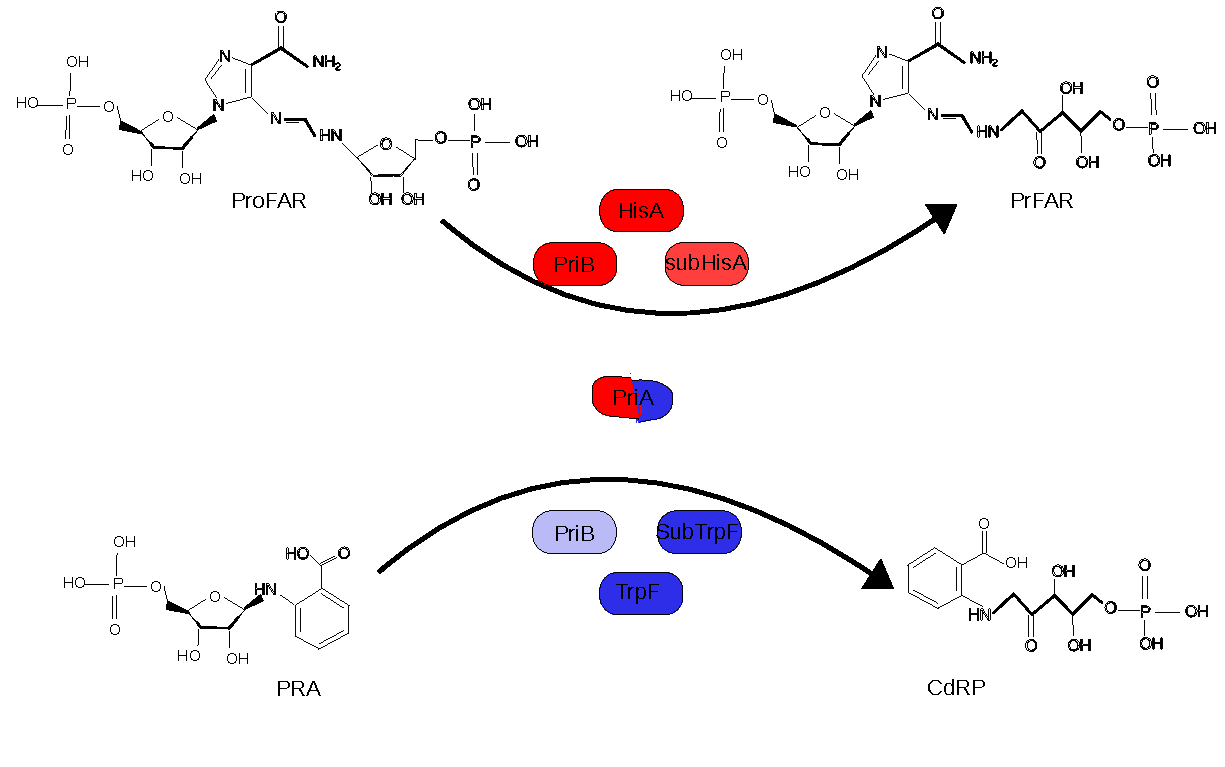
\includegraphics[angle = 0,scale = 0.6]{PriA.pdf}
\caption[PriA isomeriza los sustratos PRA y ProFAR ]{\footnotesize{PriA cataliza la isomerización  de los sustratos nativos ProFAR y PRA. Convertir ProFAR es un paso de la síntesis de histidina catalizado por {hisA} en otros linajes bacterianos. Análogamente la isomerización de PRA es catalizada por {trpF} en otros linajes. En Actinobacteria PriA se ha subdidvidido en subfamilias. Entre ellas subHisA, que se ha subfuncionalizado a la función HisA, subTrpF que se ha subfuncionalizado a la función TrpF y finalmente PriB, que aún retiene la función TrpF pero con baja actividad catalítica.  }}
\label{fig:priAFigure}
\end{figure}

Los operones his y trp de histidina {[}@fondi\_evolution\_2009{]} y
triptofano {[}@merino\_evolution\_2008{]} respectivamente, participantes
del metabolismo de aminoacidos estan ampliamente distribuidos en los
organismos bacterianos. En Actinobacteria la familia promiscua PriA
participa en ambas rutas biosinteticas \autoref{fig:priAFigure}, para su
estudio se han generado datos bioquímicos \autoref{tab:cineticos},
genómicos y estructurales. En bacterias gram negativas estan presentes
los operones his y trp y en lugar de PriA su familia homologa HisA. PriA
comprende un conjunto de subfamilias en Actinobacteria. En
\emph{Streptomyces}, el gen \emph{trpF} se desplaza de la vecindad
genomica de trp, con lo que el homologo de hisA gana promiscuidad aunque
con baja actividad de TrpF, a esta subfamilia se le llama PriB
{[}@verduzco-castro\_co-occurrence\_2016{]}. En otras Actinobacterias
trpF se pierde totalmente y la familia homologa de HisA, se vuelve
promiscua {[}@baronagomez\_occurrence\_2003{]} realizando tanto la
funcion quimica correspondiente a HisA como la de TrpF. Finalmente en la
familia subHisA se pierde la funcion TrpF debido posiblemente a la
ganancia del operon trp completo {[}@noda-garcia\_evolution\_2013{]} y
en la familia subtrpF se conserva solo a la funcion TrpF debido a la
perdida del operon his {[}Juarez vazquez et al 2015 in prep{]}. Existen
al menos 43 familias de Actinobacteria sin explorar respecto a la
funcionalidad de PriA. En la \autoref{tab:cineticos} se muestra la
constantes catalíticas de PriA estimadas en diferentes organismos para
estos dos sustratos.

\clearpage    

\begin{landscape}  
Table: Capacidad catalítica respecto a PRA y ProFAR de miembros de la familia PriA \label{tab:cineticos} 
$$
\resizebox{\columnwidth}{!}{%
\begin{tabular}{ l c r c c c c c c c l}
\hline \\ [-1.5ex]
Fuente  &Familia & HisA $in\hspace{.1cm}vivo$ &TrpF $in\hspace{.1cm}vivo$ & $K{cat}^{ProFAR}[M^{-1}s^{-1}]$ & $Km^{ProFAR}[\mu M]$& $\frac{K{cat}}{Km} ProFAR$ & $K{cat}^{PRA}[M^{-1}s^{-1}]$ & $Km^{PRA}[\mu M]$  &  $\frac{Kcat}{Km} PRA $  &Referencia  \\ [1ex]
\hline \\ [-1.5ex]  
\textit{Escherichia} \textit{coli}         & HisA &- &- & 1.6 & 4.9 & 3.1 & -   & -   & 0   & Henn-Sax 2002 \\ [1ex]  
\textit{Escherichia}  \textit{coli}        &TrpF  &- &- &-    &-    &0    & 12.2& 34.5& 2.82& Sterner 1996 \\ [1ex]    
\textit{Mycobacterium} \textit{tuberculosis} &PriA&-&-&19&0.23&12&21&3.6&0.17& Due 2011\\ [1ex]    
\textit{Mycobacterium}  \textit{smegmatis} &PriA&*&*& 2.6 ± 0.5 & 0.85 $ \pm $ 0.04 &0.33& 7.9 $ \pm $  2.4& 3.1 $ \pm $0.43  &0.39& Verduzco-Castro 2016 \\ [1ex]   
\textit{Streptomyces} \textit{globisporus}  &PriA&*&*& 4.2 ± 0.8& 0.74 ± 0.03 &0.18& 11 ± 1.0 & 3.8 ± 0.2 &0.34& Verduzco-Castro 2016\\ [1ex]  
\textit{Streptomyces} \textit{coelicolor} &PriA&-&-& 3.6 ± 0.7 & 1.3 ± 0.2 &0.4& 5.0 ± 0.08 & 3.4 ± 0.09 &0.7& Noda-Garcia 2010\\ [1ex]   
\textit{Streptomyces} \textit{ipomoeae}  &PriB&*&*& 3.8 ± 0.2 & 0.82 ± 0.02 &0.21& 60.8 ± 1.1&  8.25 ± 0.4&0.14& Verduzco-Castro 2016\\ [1ex]   
\textit{Streptomyces} sp. Mg1  &PriB&*&*& 13.2 ± 3.4 &0.92 ± 0.19 &69&129.6 ± 34 &0.29 ± 0.04&0.0022&Verduzco-Castro 2016\\ [1ex]  
\textit{Streptomyces} sp. C&PriB&*&*&11.4 ± 3.4 &2.53 ± 0.74 &0.22&149. 9 ± 29& 1.4 ± 0.12 &9&Verduzco-Castro 2016\\ [1ex]    
\textit{Streptomyces} \textit{sviceus} &PriB&*&*&3.9 ± 0.89 &0.69 ± 0.04 &0.18&24.5 ± 4.0& 1.6 ± 0.29 &67&VVerduzco-Castro 2016\\ [1ex]   
\textit{Corynebacterium} \textit{diphteriae} &subHisA&-&-&4.4 ± 0.5&2.6 ± 0.3&0.59&&&0& Noda-Garcia 2013\\ [1ex]    
\textit{Corynebacterium} \textit{jeikeium} &PriA&-&-&2.3 ± 0.2&0.9 ± 0.08&0.39&5.1 ± 1.0&1.6 ± 0.16&0.31& Noda-Garcia 2013\\ [1ex]    
\textit{Corynebacterium} \textit{striatum} &subHisA&-&-&6.9 ± 0.7&2.1 ± 0.5&0.3&&&0& Noda-Garcia 2013 \\ [1ex]    
\textit{Corynebacterium} \textit{diphteriae}  L48I-F50L-T80S&subHisA&&&4.5 ± 1.5&0.6 ± 0.08&0.13&133 ± 10&0.05 ± 0.01&0.0004&NNoda-Garcia 2013\\ [1ex]    
\textit{Actinomyces} \textit{urogenitalis} DSM 15434&PriB&*&*&2.1 ± 0.5 &1.8 ± 0.2 &0.9&26.3 ± 6.3& 0.37 ± 0.09 &14&Verduzco-Castro 2016\\ [1ex]   
\textit{Actinomyces} \textit{odontolyticus}  ATCC 17982&subTrpF&&*&-&-&0&&&0.02&Juarez-Vazquez 2017\\ [1ex]    
\textit{Actinomyces} \textit{oris} K20 BABV01&PriA&&&&&0.02&&&0.01&Juarez-Vazquez 2017\\ [1ex]    
\textit{Actinomyces} sp. oral taxon 171 str. F0337&PriA&&&&&0.01&&&4&Juarez-Vazquez 2017\\ [1ex]    
\textit{Actinomyces} sp. oral taxon 848 str. F0332&subTrpF&&*&-&-&0&&&0.0001&Juarez-Vazquez 2017\\ [1ex]    
\textit{Actinomyces} \textit{urogenitalis} DSM 15434&PriA&&&&&0.01&&&0.02&Juarez-Vazquez 2017\\ [1ex]    
\textit{Bifidobacterium} \textit{adolescentis} L2-32&PriA&*&*&&&0.2&&&0.1&Juarez-Vazquez 2017\\ [1ex]    
\textit{Bifidobacterium} \textit{gallicum} DSM 20093 &PriA&*&*&&&0.1&&&0.04&Juarez-Vazquez 2017\\ [1ex]    
\textit{Bifidobacterium} \textit{longum} ATCC 15697&PriA&*&*&&&0.1&&&0.3&Juarez-Vazquez 2017\\ [1ex]    
Camera CAM1&Metagenoma&&&1.7 ± 0.1&0.3 ± 0.03&0.2&40 ± 7&3.5 ± 0.04&0.09&Noda-Garcia 2015\\ [1ex]    
CAM1 A81G&Metagenoma&&&1.7 ± 0.2&0.1 ± 0.01&0.06&32.2 ± 1.7&1.9 ± 0.1&0.06&Noda-Garcia 2015\\ [1ex]    
CAM1 A81S&Metagenoma&&&4.0 ± 0.9&0.2 ± 0.03&0.04&23.5 ± 6.5&0.5 ± 0.1&0.02&Noda-Garcia 2015\\ [1ex]    
CAM2&Metagenoma&&&n.d.&n.d.&0&n.d.&n.d.&0&Noda-Garcia 2015\\ [1ex]    
PriA Ancestral&Ancestral&&&9.4±1.6&0.3±0.009&0.03&4.3±0.4&0.6±0.02&0.13&Verduzco, Noda, sin publicar\\ [1ex]    
PriA SubHisA&Ancestral&&&3.7±1.01&0.5±0.03&0.1&-&-&0&Verduzco, Noda, sin publicar\\ [1ex]    
SubHisA Ancestral&Ancestral&&&6.3±0.7&0.15±0.03&0.02&-&-&0&Verduzco, Noda, sin publicar\\ [1ex]    
SubHisA PriA&Ancestral&&&27.7±3.4&0.05±0.005&2&167.82&0.03±0.002&0.0001&Verduzco, Noda, sin publicar\\ [1ex]    
\textit{Streptomyces} \textit{acidiscabies}&&0&0&163.6&0.1&&&&&Verduzco*\\ [1ex]  
\textit{A} \textit{visco} &&&46&1.37&36&3.4&&&&Juárez*\\ [1ex]  
\hline \\ [-1.5ex]
\hline
\end{tabular}
}
\label{tab:cineticos}  
%}
$$   
\end{landscape}

\normalsize

\subsection{Modelos computacionales}\label{modelos-computacionales}

Para desarrollar herramientas se adoptó el enfoque de los contenedores
bioinformáticos, todo el código fue depositado y documentado en GitHub y
distribuido a través de un contenedor Docker

\clearpage


\end{document}
